% !TeX root = document.tex
% !TeX encoding = UTF-8 Unicode

\section{Introdução}%
\label{introducao}

Visando a continuidade do trabalho iniciado na disciplina de Análise de Sistemas
Lineares, a planta utilizada é um massa-mola em plano inclinado. O objetivo do
sistema é o controle da posição da massa através do controle da angulação do
plano onde ela se encontra. Uma figura ilustrativa do sistema pode ser vista
em~\ref{fig:plant}.

\begin{figure}[H]
	\centering
	\captionsetup{justification=centering}
	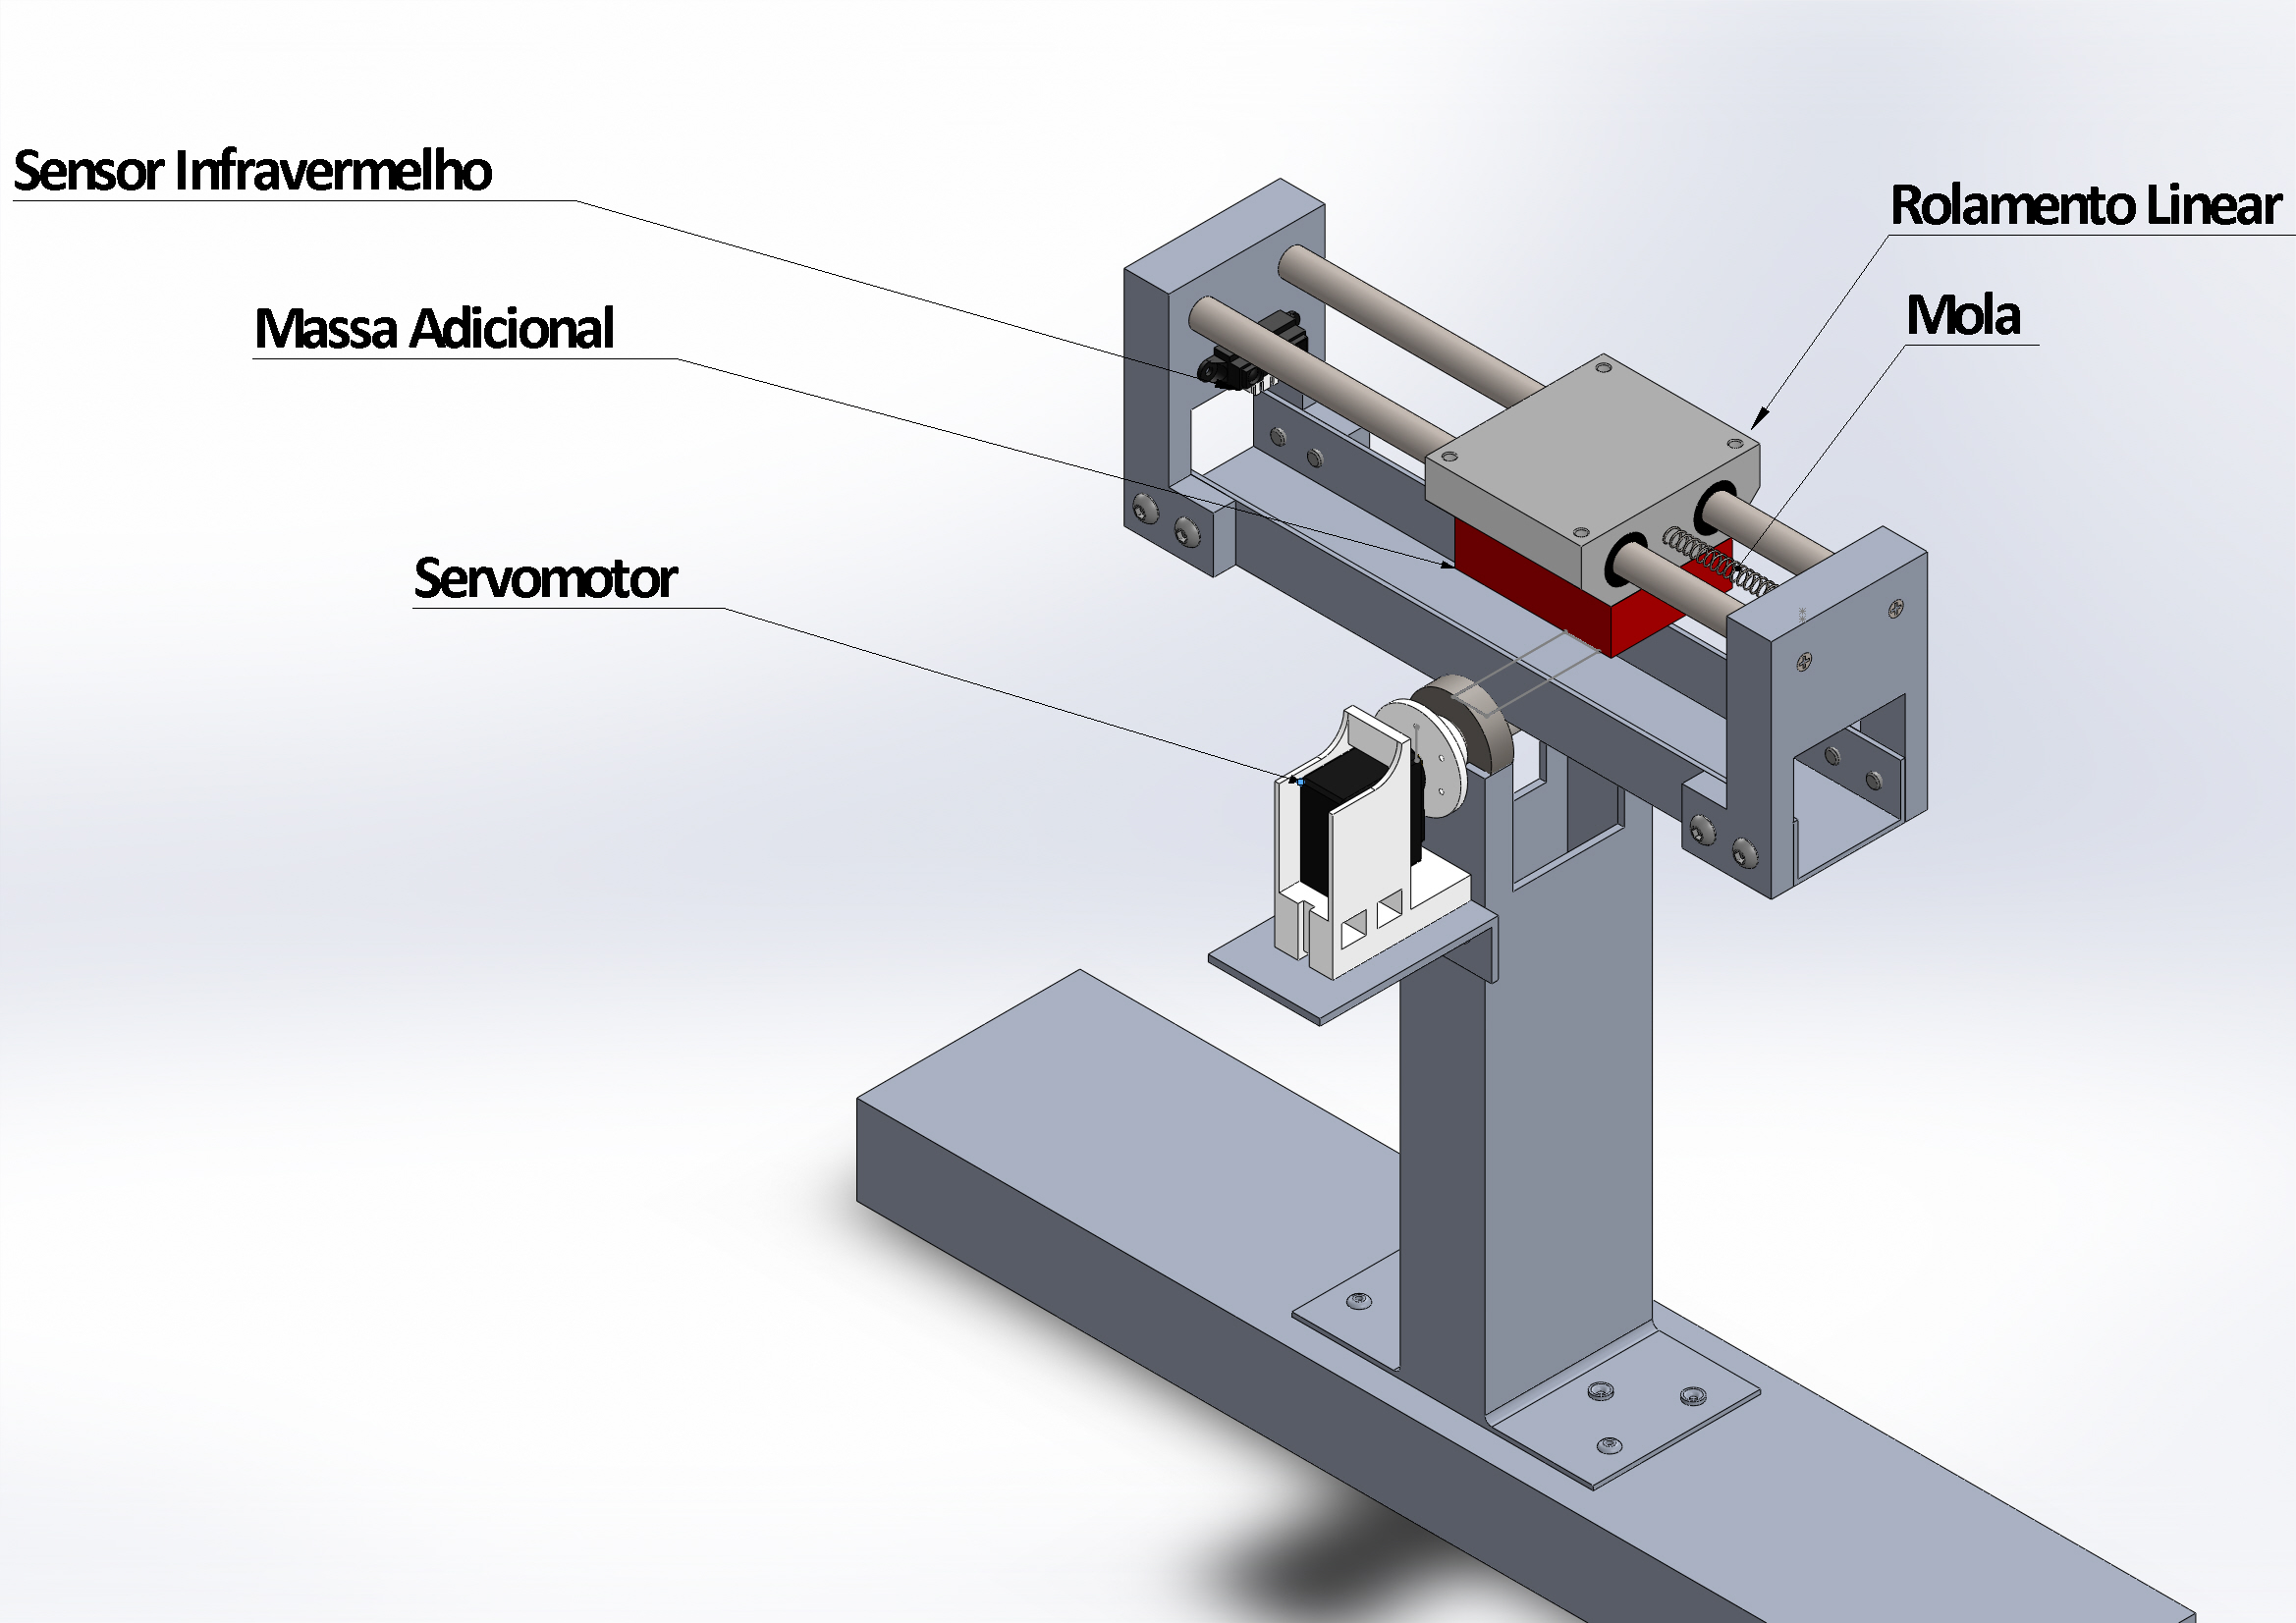
\includegraphics[width=0.8\linewidth]{imgs/planta}
	\caption{Sistema massa-mola em plano inclinado}%
	\label{fig:plant}
\end{figure}

Para medir a distância utiliza-se o sensor de distância infravermelho
GP2Y0A21YK0F. Trata-se de um sensor não linear capaz de medir de 5 a 150 cm, com
saída de 0 a 5V, inversamente proporcional à distância. Para controlar a
angulação utiliza-se um motor de passo Tower Pro MG995. Ambos são calibrados,
sendo as grandezas reais aquelas utilizadas na identificação do sistema, ou seja
a função de transferência que representa o sistema tem como entrada o ângulo do
plano e como saída a distância da massa.

As limitações físicas da planta são 0 a 20cm e 0 a 180 graus. No entanto, os
limites dos ângulos foram alterados de forma a evitar movimentações na área de
folga do motor, de compressão da mola e que force o plano contra a haste,
resultando em saturações em 30º e 120º.
